
% THIS IS SIGPROC-SP.TEX - VERSION 3.1
% WORKS WITH V3.2SP OF ACM_PROC_ARTICLE-SP.CLS
% APRIL 2009
%
% It is an example file showing how to use the 'acm_proc_article-sp.cls' V3.2SP
% LaTeX2e document class file for Conference Proceedings submissions.
% ----------------------------------------------------------------------------------------------------------------
% This .tex file (and associated .cls V3.2SP) *DOES NOT* produce:
%       1) The Permission Statement
%       2) The Conference (location) Info information
%       3) The Copyright Line with ACM data
%       4) Page numbering
% ---------------------------------------------------------------------------------------------------------------
% It is an example which *does* use the .bib file (from which the .bbl file
% is produced).
% REMEMBER HOWEVER: After having produced the .bbl file,
% and prior to final submission,
% you need to 'insert'  your .bbl file into your source .tex file so as to provide
% ONE 'self-contained' source file.
%
% Questions regarding SIGS should be sent to
% Adrienne Griscti ---> griscti@acm.org
%
% Questions/suggestions regarding the guidelines, .tex and .cls files, etc. to
% Gerald Murray ---> murray@hq.acm.org
%
% For tracking purposes - this is V3.1SP - APRIL 2009

\documentclass{acm_proc_article-sp}

\usepackage{multirow}
\usepackage{subfigure}
\usepackage{graphicx}
\usepackage{graphics}
\usepackage{rotating}
\usepackage{verbatim}
\usepackage{float}
\usepackage{url}
\usepackage{tabularx}
\usepackage{amsmath}
\usepackage{listings}
\usepackage{color}
\definecolor{javared}{rgb}{0.6,0,0} % for strings
\definecolor{javagreen}{rgb}{0.25,0.5,0.35} % comments
\definecolor{javapurple}{rgb}{0.5,0,0.35} % keywords
\definecolor{javadocblue}{rgb}{0.25,0.35,0.75} % javadoc
 
\lstset{language=Java,
basicstyle=\ttfamily,
keywordstyle=\color{javapurple}\bfseries,
stringstyle=\color{javared},
commentstyle=\color{javagreen},
morecomment=[s][\color{javadocblue}]{/**}{*/},
%numbers=left,
numberstyle=\tiny\color{black},
stepnumber=2,
numbersep=10pt,
tabsize=4,
showspaces=false,
showstringspaces=false}



\restylefloat{table}

\hyphenation{op-tical net-works semi-conduc-tor}



\begin{document}



\title{Automated Discovery of Failure Domain+ and Daikon to Analyse Failure Boundaries}


\numberofauthors{2} %  in this sample file, there are a *total*
% of EIGHT authors. SIX appear on the 'first-page' (matting
% reasons) and the remaining two appear in the \additionalauthors section.
%
\author{
% You can go ahead and credit any number of authors here,
% e.g. one 'row of three' or two rows (consisting of one row of three
% and a second row of one, two or three).
%
% The command \alignauthor (no curly braces needed) should
% precede each author name, affiliation/snail-mail address and
% e-mail address. Additionally, tag each line of
% affiliation/address with \affaddr, and tag the
% e-mail address with \email.
%
% 1st. author
\alignauthor
Mian Asbat Ahmad\\
       \affaddr{Department of Computer Science}\\
       \affaddr{The University of York}\\
       \affaddr{York, United Kingdom}\\
       \email{mian.ahmad@york.ac.uk}
% Please Dr. Manuel, add your abb details. I am not able to create table here because of the format. Thanks.
\alignauthor
Manuel Oriol \\
       \affaddr{Department of Computer Science}\\
       \affaddr{The University of York}\\
       \affaddr{York, United Kingdom}\\
       \email{manuel.oriol@york.ac.uk}
}



\maketitle
\begin{abstract}
This paper verifies the accuracy of invariants generated automatically by Daikon and suggests how to improve their quality. To achieve this, it uses a newly developed Automated Discovery of Failure Domain+ (ADFD+) technique. ADFD+ is a testing frame-work which after identifying a failure searches its surrounding to find its domain within the set range. The result obtained is presented graphically on a two-dimension chart.

Several error-seeded one and two-dimensional numerical programs with point, block and strip failure domain were evaluated independently for 30 times by both ADFD+ and Daikon. On analysis of results, it is found that where Daikon generates the correct invariants, it was not good enough to identify the exact failure boundaries.

It is concluded that the invariants generated by Daikon can be made further effective if the boundary values of the failure domain identified by ADFD+ are passed to the Daikon as test cases.

\end{abstract}

%A category including the fourth, optional field follows...
%\category{D.2.5}{Software Engineering}{Metrics}[complexity measures, performance measures]

%\terms{Comparison, Verification, }

\keywords{software testing, automated random testing} % NOT required for Proceedings





%%%%%%%%%%%%%%%%%    INTRODUCTION   %%%%%%%%%%%%%%%%%%%%

\section{Introduction}\label{sec:intro}
Testing is the most widely used and essential method in verification and validation process. Ample efforts have been made to improve its effectiveness and efficiency. Testing is effective if it finds maximum number of faults in minimum number of test cases. Testing is efficient if it executes maximum number of test-cases in minimum possible time. Upgrading existing and developing new improved test strategies can increase test effectiveness. While automating a single component or complete system increases its efficiency.

Boundary Value Analysis~\cite{radatz1990ieee} and Daikon~\cite{ernst2007daikon} are among the several approaches used to increase testing effectiveness and efficiency. In Boundary Value Analysis (BVA) technique test data from boundaries of domain are added because it is assumed that errors often reside along the boundaries. Similarly, Daikon is a tool, which saves precious testers time by automatically generating likely program invariants.

However, the approaches can adversely affect testing process if wrong boundaries or invariants are taken into consideration. It is therefore motivating to measure the degree of correctness of auto-generated invariants by Daikon in the case of point, block and strip failure domain. To assess this, we set up and performed several experiments and analysed the results derived from the error-seeded programs tested independently with ADFD+ and Daikon. ADFD+ stands for Automated Discovery of Failure Domain+ is an extended test framework based on our previous approach Automated Discovery of Failure Domain (ADFD). For more details of ADFD please see~\cite{ahmad2013adfd}.  

The main contributions of the article are:
\begin{itemize}
\item \textbf{ADFD+:} It extends our previously proposed ADFD strategy. The new strategy improves the search algorithm of ADFD and makes the report more intuitive.
\item \textbf{Implementation of ADFD+:} The new ADFD+ strategy is implemented and integrated in the York Extensible Testing Infrastructure (YETI).
\item \textbf{Evaluation:} It evaluate the reports generated by ADFD+ and Daikon about the boundaries of the failure domains in the error-seeded programs. It is found that where Daikon was able to find the failure, it was not able to identify its domain boundary as accurately as ADFD+.
\item \textbf{Future work:} It gives ideas of further application of ADFD+, such as finding and plotting of failures in multi-dimensional non-numerical programs using multi-dimensional graphs. 
% A case study suggesting that boundaries are properly recognized by Daikon and ADFD+ or Daikon lake .... etc.
\end{itemize}
%The rest of this paper is organised as follows: \\ Section~\ref{sec:adfd} describes the ADFD+ strategy. Section~\ref{sec:imp} presents implementation of the ADFD+ strategy. Section~\ref{sec:eval} explains the experimental setup. Section~\ref{sec:res} shows results of the experiments. Section~\ref{sec:discussion} discusses the results. Section~\ref{sec:rw} presents related work and Section~\ref{sec:conc}, concludes the study.


%In the later part we plot the domain on the basis of invariants generated by Daikon and compare both the domains.

%%%%%%%%%%%%%%%%%    Background   %%%%%%%%%%%%%%%%%%%

\section{Preliminaries}
A number of empirical evidence confirms that failure revealing test cases tend to cluster in contiguous regions across the input domain~\cite{finelli1991nasa, schneckenburger2007towards, white1980domain}. According to Chan et al.~\cite{chan1996proportional} the clusters are arranged in the form of point, block and strip failure domain. In the point domain the failure revealing inputs are stand-alone that are spread through out the input domain. In block domain the failure revealing inputs are clustered in one or more contiguous areas. Finally, in strip domain the failure revealing inputs are clustered in one long elongated area.  Figure~\ref{fig:failurePatterns} shows the failure domains in two-dimensional input domain. 

\begin{figure}[ht]                                    
\centering
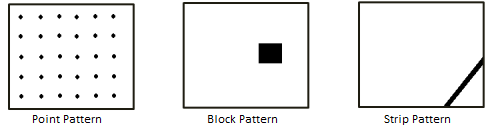
\includegraphics[width= 8cm,height=3cm]{ART_Patterns.png}
\caption{Failure domains across input domain~\cite{chan1996proportional}}
\label{fig:failurePatterns}
\end{figure}

%In Section~\ref{sec:adfd+} we describe the ADFD+ framework that can find the failure, its domain and plot the domain up to the specified range in a graphical form. Experiments confirms the successful working of ADFD+.


 

%%%%%%%%%%%%%%%%%    ADFD+   %%%%%%%%%%%%%%%%%%%

\section{Automated Discovery of Failure Domain+}\label{sec:adfd+}
ADFD+ is an improved and extended form of our previously developed Automated Discovery of Failure Domain technique~\cite{ahmad2013adfd}. The ADFD+ is an automated framework that finds the failures and their domains within a specified range and present them on a graphical chart. Following are the main improvements of ADFD+ over ADFD.

\begin{itemize}
\item ADFD+ generates a single Java file dynamically at run time to plot the failure domains instead of one Java file per failure as in ADFD. This saves a lot of execution time and makes the process quicker.

\item ADFD+ uses (x, y) vector series to represent failure domains as opposed to the (x, y) line series in ADFD. The vector series allows more flexibility and clarity to represent a failure and its domain.   

\item ADFD+ takes a single value as range with in which the strategy search for a failure domain whereas ADFD takes two values for lower and upper bound representing x and y-axis respectively.

\item In ADFD+, the algorithm of dynamically generated Java file, created at run-time, after a failure is detected is made more simplified and efficient.

\item In ADFD+, the failure domain is focused in the graph, which gives a clear view of, pass and fail points. The points are also labelled for simplification as shown in Figure~\ref{fig:Workflow}. 

%The difference in representation of fault by ADFD and ADFD+ can be seen in figure .... Figure x is generated by ADFD with lower bound as ... and upper bound as ... While Figure Y is generated by ADFD+ with range ... for the same program given in appendix a. 
\end{itemize}


%%%%%%%%%%%%%%%%%%%%

\subsection{Workflow of ADFD+}
ADFD+ is an automatic process and all the user has to do is to specify the program to test and click the $Draw Fault Domain$ button. The default value for range is set to 5, which means that ADFD+ will search 83 values around the failure. On clicking the button YETI is executed with ADFD+ strategy to search for a failure in two-dimension program. On finding a failure the ADFD+ strategy creates a Java file which contain calls to the program on the failing value and its surrounding values within the specified range. The Java file is compiled and executed and the result is analysed to check for pass and fail values. Pass and fail values are stored in pass and fail text files respectively. At the end of test, all the values are plotted on the graph with pass values in blue and fail values in red colour as shown in the Figure~\ref{fig:Workflow}.


%Instead of front end give workflow. It will make more sense. Change the code of the program

\begin{figure}[ht]
\centering
\includegraphics[width= 8.5cm,height=7cm]{adfdPlusWorkflow.png}
\caption{Workflow of ADFD+}
\label{fig:Workflow}
\end{figure}


%%%%%%%%%%%%%%%%%%%%
%ADFD+ is an extension of ADFD's algorithm with more accuracy to find and clarity to plot the failure domain on a graphical chart. Deriving failure domains using ADFD+ is a one click process and all the tester needs to input is the class to test and the range-value for which to search around the found failure. 
%%%%%%%%%%%%%%%%%%%%

\subsection{Implementation of ADFD+}
The ADFD+ technique is implemented in YETI. The tool YETI is available in open-source at \url{http://code.google.com/p/yeti-test/}. We give a brief overview of YETI with the focus on the parts relevant to the implementation of ADFD+ strategy. For verification of ADFD+ strategy in YETI, a program is used as an example to illustrate the working of ADFD+ strategy. Please refer to~\cite{Oriol2011yeti, oriol2012random, oriol2010testing, oriol2010yeti} for more details on YETI. 

YETI is a testing tool developed in Java that test programs using random strategies in an automated fashion. YETI meta-model is language-agnostic which enables it to test 
programs written in functional, procedural and object-oriented languages. 

YETI consists of three main parts including core infrastructure for extendibility through specialization, strategies section for adjustment of multiple strategies and 
languages section for supporting multiple languages. Both the languages and strategies sections have a pluggable architecture to easily incorporate new strategies and 
languages making YETI a favourable choice to implement ADFD+ strategy. YETI is also capable of generating test cases to reproduce the failures found during the test session. 
The strategies section in YETI contains all the strategies including random, random+ and DSSR to be selected for testing according to the specific needs. The default test 
strategy for testing is random. On top of the hierarchy in strategies, is an abstract class YetiStrategy, which is extended by YetiRandomPlusStrategy and is further, extended to get 
ADFD+ strategy.

\begin{figure*}[ht]
\centering
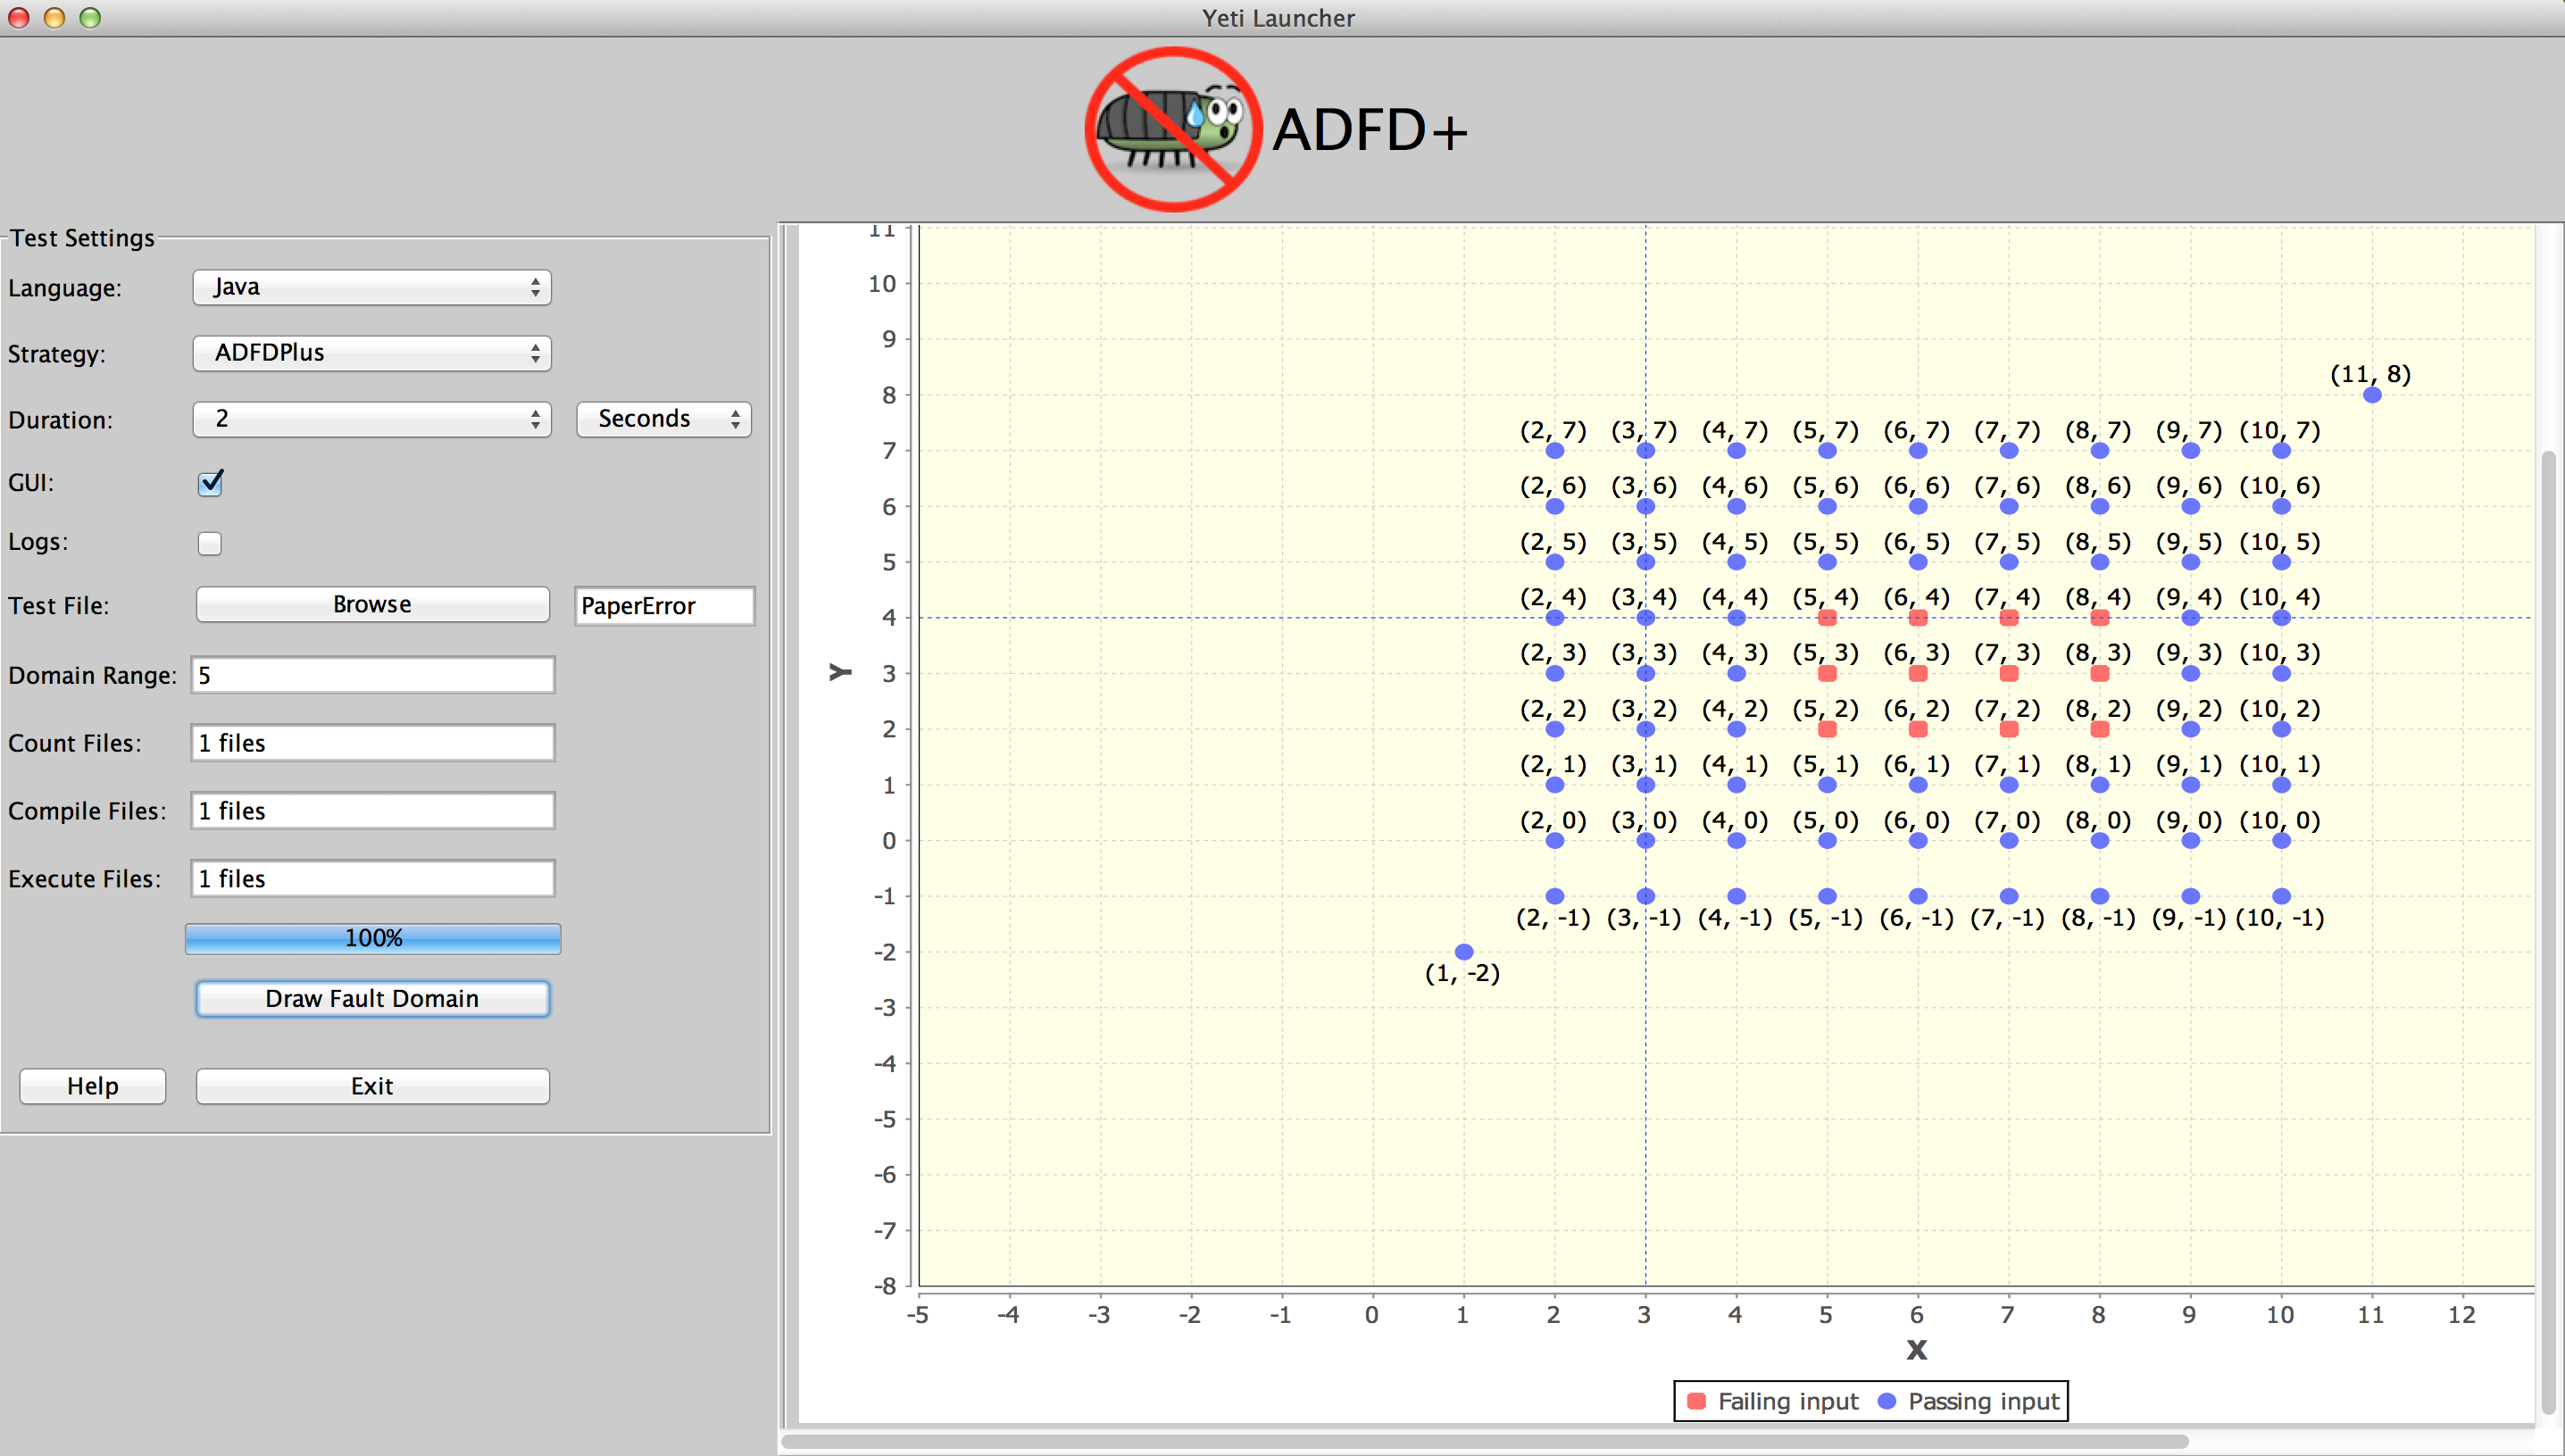
\includegraphics[width=17.5cm,height=11cm]{exampleError.png}
\caption{The output of ADFD+ for the above code.}
\label{fig:adfdPlusExample}
\end{figure*}

\subsection{ADFD+ by an example}
In this section we describe the working of ADFD+ with a motivating example. Suppose we have the following class name $Error$ under test. According to the code, the value of variable $x$ between 5 to 8 and the value of variable $y$ between 2 to 4 triggers an $ArithmeticException$ failure.

\begin{lstlisting}

public class Error {

  public static void Error (int x, int y){

    int z;

    if (((x>=5)&&(x<=8))&&((y>=2)&&(y<=4)))
		 {
			 z = 50/0;
		 }
   } 
}
\end{lstlisting}

On execution, the ADFD+ strategy tests the class with the help of YETI and finds the first failure at x = 6 and y = 3. Once a failure is identified ADFD+ uses the surrounding values around it to find a failure domain. The range of surrounding values is limited to the value set by the user in the $Domain Range$ variable. When the value of $Domain Range$ is 5, ADFD+ evaluates total of 83 values of $x$ and $y$ around the found failure. All evaluated (x, y) values are plotted on a two-dimensional graph with red filled circles indicating fail values and blue filled circles indicating pass values. Figure~\ref{fig:adfdPlusExample} shows that the failure domain forms a block pattern and the boundaries of the failure are $(5, 2), (5, 3),(5, 4), (6, 2), (6, 4), (7, 2), (7, 4), (8, 2), (8, 3), (8, 4)$. 





%%%%%%%%%%%%%%%%%%%%%%%%%%%%%%%%%%%%%%%%%%%%%%%%%

\section{Daikon}
Daikon~\cite{ernst2007daikon} is a tool, which uses machine-learning technique to automatically generate likely invariants of the program written in C, C++, Java and Pearl. Daikon takes as input the program and few test cases written manually or generated by an automated tool. It executes the test cases on the program under test and observes the values that the program computes. At the end of the test session it reports the properties that were true over the observed executions. Daikon can process the generated invariants to mitigate non-interesting and redundant invariants. Daikon can also inserts the generated invariants in to the source code as assertions. Daikon's output can be useful in understanding program, generating invariants, predicting incompatibilities in component integration, automating theorem proving, repairing inconsistent data structures and checking the validity of data streams.




%%%%%%%%%%%%%%%%%    EVALUATION   %%%%%%%%%%%%%%%%%%%%


\section{Evaluation}\label{sec:eval}
Because of using error-seeded one and two dimensional numerical programs, we were aware of the failure domain present in each program. The correct identification and presentation of the failure domain by ADFD+ prove the correct working of ADFD+. We then evaluated the same program by Daikon and plot its results. The unit test cases required by Daikon for generating invariants were generated using Randoop~\cite{}. YETI being capable of generating the test cases is not used for this step to keep the second completely independent from first. 

\subsection{Research questions}
For evaluating Daikon, the following research questions have been addressed in this study:
\begin{enumerate}
\item If Daikon is capable of generating invariants to identify the failure?
\item If Daikon is capable of generating invariants that identify the failure domain?
\item If Daikon is capable of correctly identifying the boundaries of the failure domain?
\end{enumerate}

\subsection{Experimental setup}
To evaluate the invariants generated by Daikon in case of point, block and strip failure domain, we performed testing of several error seeded one and two-dimensional numerical programs written in Java. The programs were divided in to two sets. Set A and B contains one and two-dimensional programs. Each program is injected with point, block or strip failure domain. Every program is tested independently for 20 times by both ADFD+ and Daikon. The external parameters were kept constant in each test run and the initial test cases required by Daikon for generating invariants were generated by using an automated testing tool Randoop. The code for the programs under test is given in Appendix~\ref{} while the test details are presented in Table~\ref{table:Results}. The effect of increased number of test cases is also shown in column .. of Table~\ref{table:Results}.

%Every class is evaluated through $10^5$ calls in each test session of ADFD+.
%\footnote{The total number of tests is equal to $60\times 30\times 3 \times 10^5 = 540\times10^6~tests$.} 
Because of the absence of the contracts and assertions in the code, similar approach as used in previous study ~\cite{ahmad2013adfd, Oriol2012} is followed using undeclared exceptions to compute failures.

All tests are performed with a 64-bit Mac OS X Lion Version 10.7.4 running on 2 x 2.66 GHz 6-Core Intel Xeon processor with 6 GB (1333 MHz DDR3) of RAM. YETI runs on top of the Java\texttrademark  SE Runtime Environment [version 1.6.0\_35]. The machine took approximately 100 hours to process the experiments.

\section{results}

The results are split in to four sub-sections for convenience. 

\subsection{Test of one-dimension programs by ADFD+}
In each of the 20 experiments, The ADFD+ successfully discovered and plotted the failure domains for point, block and strip pattern as shown in the Figure~\ref{}. The lower and upper bound for each experiment were kept --- and --- respectively.

\begin{figure} [H]

\subfigure[Point failure domain in one-dimension]{
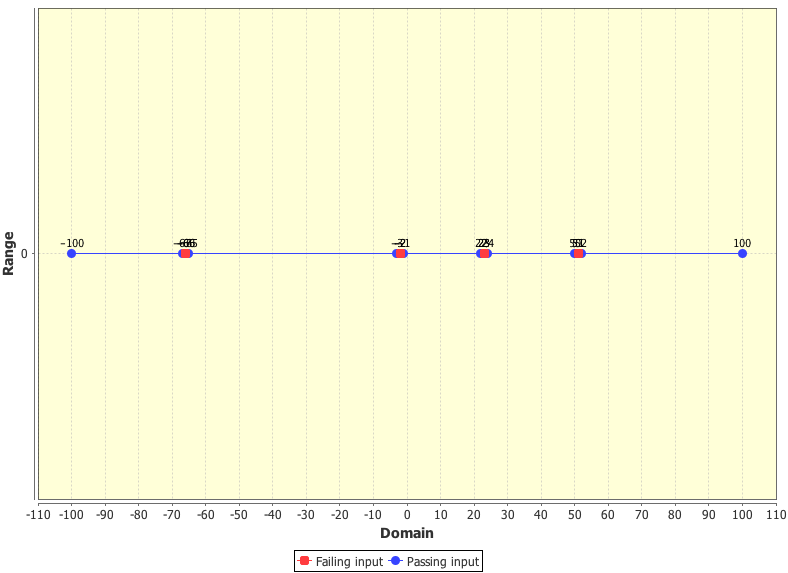
\includegraphics[width=8cm,height=6cm]{PFDOne.png}
\label{fig:PFDOne}
}
\subfigure[Block failure domain in one-dimension]{
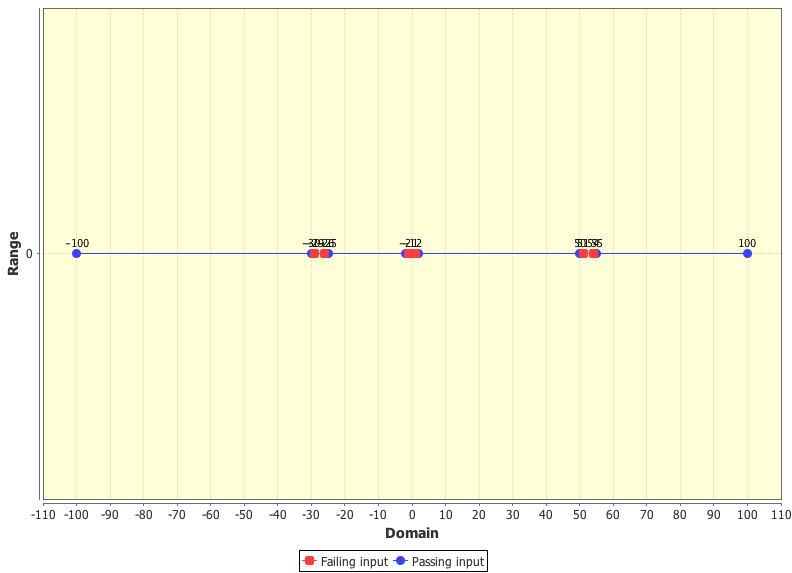
\includegraphics[width=8cm,height=6cm]{BFDOne.png}
\label{fig:BFDOne}
}
\subfigure[Strip failure domain in one dimension]{
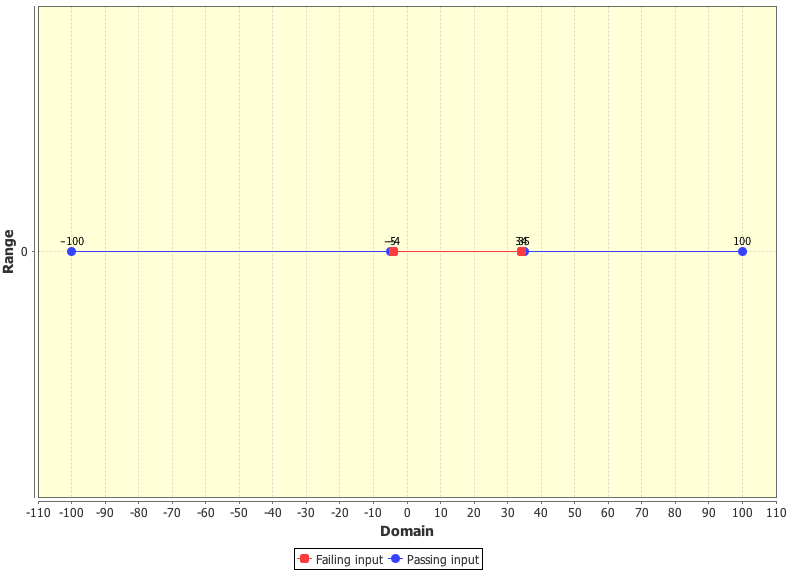
\includegraphics[width=8cm,height=6cm]{SFDOne.png}
\label{fig:SFDOne}
}
\caption{Pass and fail values of plotted by ADFD+ in three different cases of two-dimension programs}

\end{figure}




\subsection{Test of one-dimension programs by Daikon}


\subsection{Test of two-dimension programs by ADFD+}
In each of the 20 experiments, The ADFD+ once again successfully discovered and plotted the failure domain for point, block and strip failure domain as shown in the Figure~\ref{}. The range for each experiment were kept ----.

\begin{figure} [H]

\subfigure[Point failure domain in two-dimension]{
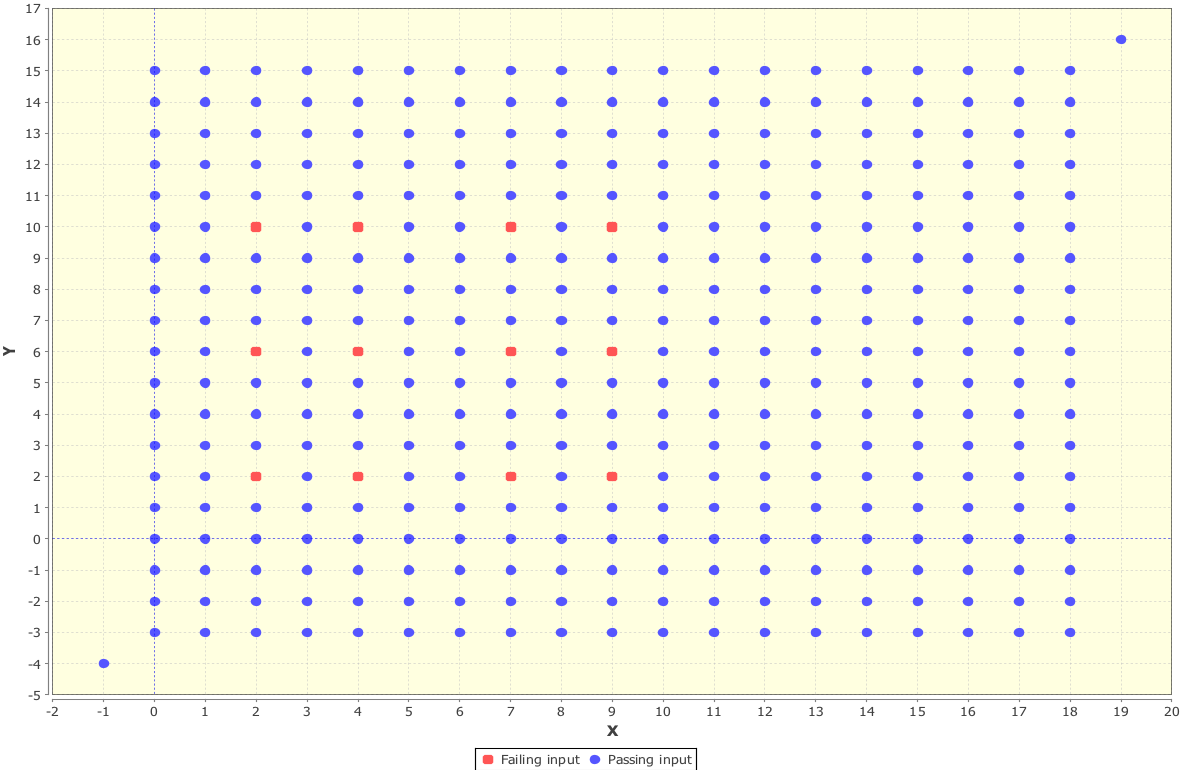
\includegraphics[width=8cm,height=6cm]{PFDTwo.png}
\label{fig:PFDOne}
}
\subfigure[Block failure domain in two-dimension]{
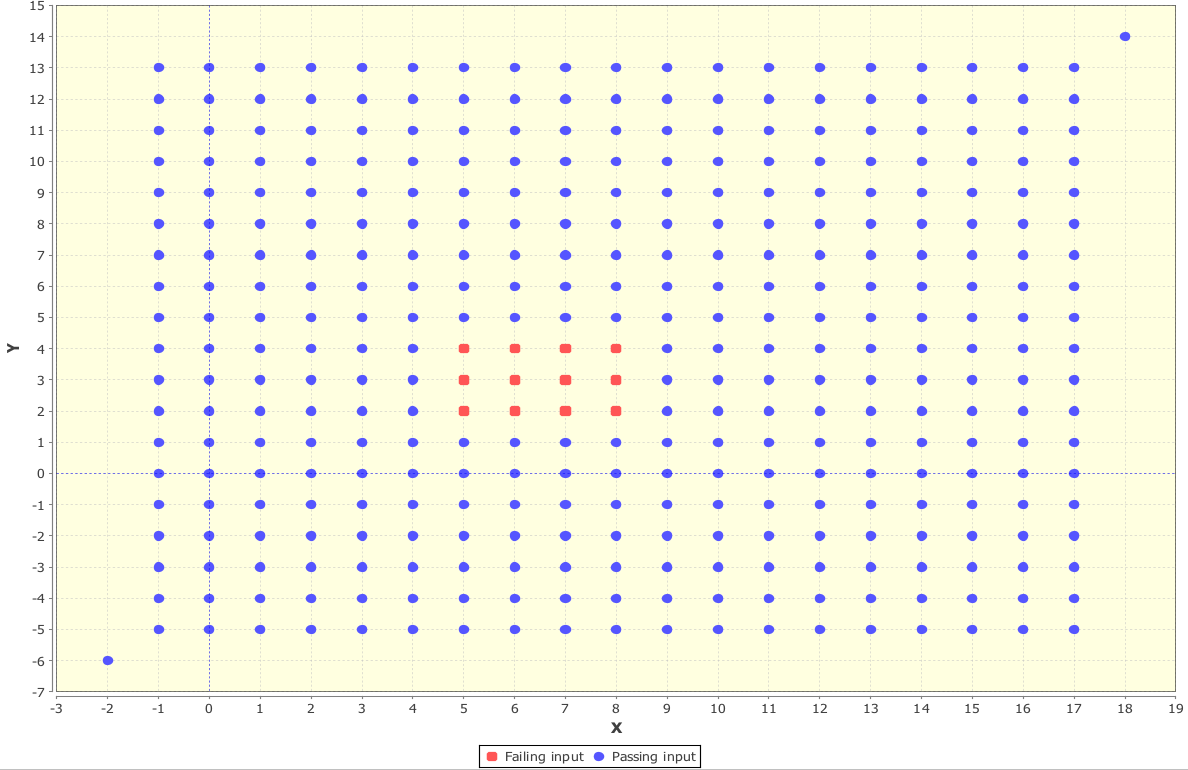
\includegraphics[width=8cm,height=6cm]{BFDTwo.png}
\label{fig:BFDOne}
}
\subfigure[Strip failure domain in two-dimension]{
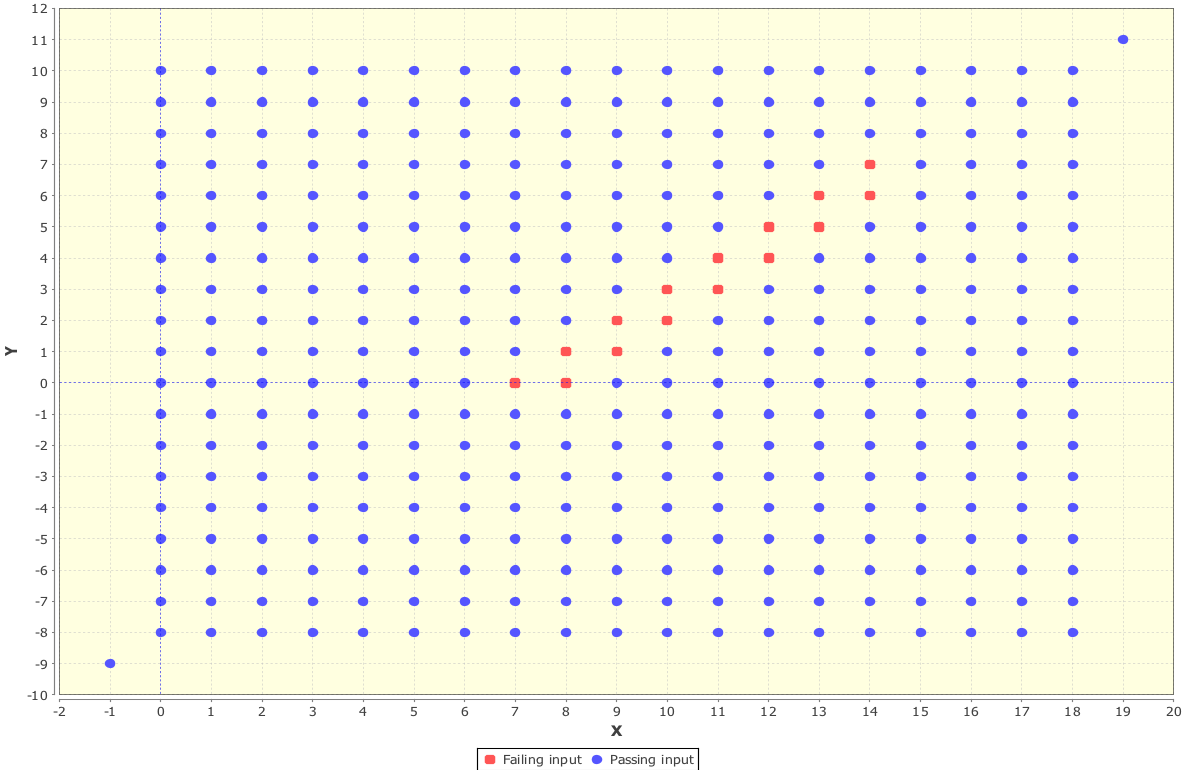
\includegraphics[width=8cm,height=6cm]{SFDTwo.png}
\label{fig:SFDOne}
}
\caption{Pass and fail values of plotted by ADFD+ in three different cases of two-dimension programs}

\end{figure}


\subsection{Test of two-dimension programs by Daikon}





%for point, block and strip of one dimensional program. Use the same programs of ADFD, same figures but analyse it again on Daikon. because ADFD and ADFD+ behave in the same way for one dimension. For point block and strip of two dimensional programs. Use adfd+ system.






\section{Discussion}
We have shown that ADFD+ is a promising technique to find a failure and using it as a focal point find the whole failure domain. We have also shown that ADFD+ can graphically draw the failure domain on a chart. The failure values are drawn in red and the pass values are drawn in green. The pictorial representation of failure domain helps in easily identifying the underlying pattern and its boundaries.

As a pilot study, we also ran an empirical study to evaluate several error-seeded programs. While it would be surprising if production programs produced much different results, it would be worthwhile to check.

More importantly, the implementation of ADFD+ for this pilot study has significant limitations in practice, as it requires only one and two dimensional numerical programs. Though it is not difficult to extend the approach to test more than two-dimensional programs containing other primitive types, it would however be difficult to plot them on the chart as the number of coordinates increases. The approach can also be extended to test object-oriented programs by implementing objects distance proposed by Ciupa et al. \cite{}. The details of such an implementation will take some effort.

The ADFD+ range value specifies how many values to test around the failure. The range can be set to any number before the test starts. The value of range is directly proportional to the time taken because the higher the range value the higher number of values to test. Higher range value also leads to a very large graph and the tester has to use the zoom feature of graph to magnify the failure region.




\section{Threats to validity}
The threats to external validity are the same, common to all empirical evaluation i.e. the degree to which the tested classes and external test generation tool (Randoop) are representative of true practice. The classes are very simple concerning failure domain in only one and two-dimensional input domain. The threats could be reduced by experiments on various types of classes and different auto test generation tools. The main threat to internal validity includes annotation of invariants that can bias our results. Error seeded classes selected in our implementation, might cause such effects. Taking in to consideration the real failures in real classes could also reduce the threat. Furthermore, testing a higher number of classes would naturally have increased the reliability of the results.

\section{Conclusion}

\section{Future Work}
We aim to extend the current approach to a larger set of real world multi-dimension programs, using real failure instead of error-seeded programs. Moreover, to plot failure domains of complex multi-dimension shapes we would also require more sophisticated graphical tool like Matlab than JFreeChart. This could also result in the formation of new failure domains of different nature instead of the only point, block and strip failure domain in one and two dimension numerical programs. 



%%%%%%%%%%%%%%%%%%%%%%%
\begin{comment}

%Results of the 60 classes tested in the study are divided in to 11 different categories as presented in ~\ref{table:categories}. 

\begin{table}[h]
\caption{Results of the 60 classes are divided into 11 categories}
\centering
\begin{tabular}{|r|l|r|}
\hline
S. No	& 	Category			& 	Result\\
\hline
1		&	DSSR > R			&	12 \\	
2		&	DSSR > R+		&	10 \\	
3		&	DSSR = R			&	5 \\	
4		&	DSSR = R+		&	7 \\	
5		&	R+ > R 			&	10 \\	
6		&	R+ < R			&	5 \\	
7		&	R+ = R			&	2 \\	
8		&	R > R+			&	4 \\
9		&	DSSR < R			&	0 \\	
10		&	DSSR < R+		&	0 \\
11		&	DSSR = R = R+	&	43 \\			
\hline
\end{tabular}
\bigskip
\label{table:categories}
\end{table}







%%%%%%%%%%%%%%%%%    DISCUSSION   %%%%%%%%%%%%%%%%%%%%

\section{Discussion}\label{sec:discussion}
In this section we discuss various factors such as the time taken, effect of test duration, number of tests, number of faults in the different strategies and the effect of finding first fault in the DSSR strategy.
\textbf{Time taken to execute an equal number of test cases:}
The DSSR strategy takes slightly more time (up to 5\%) than both pure random and random plus which may be due to maintaining sets of interesting values during the execution. We do not believe that the overhead can be reduced. 

\textbf{Effect of test duration and number of tests on the results:}
All three techniques have the same potential for finding failures. If testing is continued for a long duration then all three strategies will find the same number of unique failures and the results will converge. We suspect however that some of the unique failures will take an extremely long time to be found by using random or random+ only. Further experiments should confirm this point.


\textbf{Effect of number of faults on results:} 
We found that the DSSR strategy performs better when the number of faults is higher in the code. The reason seems to be that when there are more faults, their domains are more connected and DSSR strategy works better. Further studies might use historical data to pick the best strategy.

\textbf{Dependence of DSSR strategy to find the first unique failure early enough:}
During the experiments we noticed that if a unique failure is not found  quickly enough, there is no value added to the list of interesting values and then the test becomes equivalent to random+ testing. This means that better ways of populating failure-inducing values are needed for sufficient leverage to DSSR strategy. As an example, the following piece of code would be unlikely to fail under the current setting:

\begin{lstlisting}
public void test(float value){
 if(value == 34.4445)   10/0;
}
\end{lstlisting}

In this case, we could add constant literals from the SUT to the list of interesting values in a dynamic fashion. These literals can be obtained from the constant pool in the class files of the SUT.

In the example above the value 34.4445 and its surrounding values would  be added to the list of interesting values before the test starts and the DSSR strategy would find the unique failure right away.

\textbf{DSSR strategy and coverage:} Random strategies typically achieve high level of coverage~\cite{Oriol2010}. It might also be interesting to compare R, R+ and DSSR with respect to the achieved coverage or even to use a DSSR variant that adds a new interesting value and its neighbours when a new branch is reached.


\textbf{Threats to validity:} As usual with such empirical studies, the present work might suffer from a non-representative selection of classes.
The selection in the current study is however made through random process and objective criteria, therefore, it seems likely that it would be representative.

The parameters of the study might also have prompted incorrect results. But this is unlikely due to previous results on random testing~\cite{Oriol2012}.



%%%%%%%%%%%%%%%%%    RW   %%%%%%%%%%%%%%%%%%%%

\section{Related Work}\label{sec:rw}

Random testing is a popular technique with simple algorithm but proven to find subtle faults in complex programs and Java libraries~\cite{Pacheco2005, Csallner2004, Claessen2000a}. Its simplicity, ease of implementation and efficiency in generating test cases make it the best choice for test automation~\cite{Hamlet1994}. Some of the well known automated tools based on random strategy includes Jartege~\cite{Oriat2004}, Eclat~\cite{Pacheco2005}, JCrasher~\cite{Csallner2004}, AutoTest \cite{Ciupa2007, Ciupa2008a} and YETI~\cite{Oriol2010, Oriol2012}.

In pursuit of better test results and lower overhead, many variations of random strategy have been proposed~\cite{Chen2010, Chen2005, Chan2002, Chen2004a, Chen2003}. Adaptive random testing (ART), Quasi-random testing (QRT) and Restricted Random testing (RRT) achieved better results by selecting test inputs randomly but evenly spread across the input domain. Mirror ART and ART through dynamic partitioning increased the performance by reducing the overhead of ART. The main reason behind better performance of the strategies is that even spread of test input increases the chance of exploring the fault patterns present in the input domain.

A more recent research study \cite{Yoo2012} stresses on the effectiveness of data regeneration in close vicinity of the existing test data. Their findings showed up to two orders of magnitude more efficient test data generation than the existing techniques. Two major limitations of their study are the requirement of existing test cases to regenerate new test cases, and increased overhead due to ``meta heuristics search'' based on hill climbing algorithm to regenerate new data. In DSSR no pre-existing test cases are required because it utilises the border values from R+ and regenerate the data very cheaply in a dynamic fashion different for each class under test without any prior test data and with comparatively lower overhead. 
  
The random+ (R+) strategy is an extension of the random strategy in which interesting values, beside pure random values, are added to the list of test inputs~\cite{Leitner2007}. These interesting values includes border values which have high tendency of finding faults in the given SUT~\cite{Beizer1990}. Results obtained with R+ strategy show significant improvement over random strategy~\cite{Leitner2007}. DSSR strategy is an extension of R+ strategy which starts testing as R+ until a fault is found then it switches to spot sweeping.

%It is interesting that numerous efforts have been made to discover the fault patterns~\cite{Chen2010, Chen2005, Chan2002, Chen2004a, Chen2003}, etc. but in our knowledge, none has been published on covering/sweeping all the faults lying in a specific pattern once it has been discovered.


A common practice to evaluate performance of an extended strategy is to compare the results obtained by applying the new and existing strategy to identical programs~\cite{Gutjahr1999, Duran1984, Hamlet1990}. Arcuri et al. \cite{Arcuri2012}, stress on the use of random testing as a baseline for comparison with other test strategies. We followed the procedure and evaluated DSSR strategy against R and R+ strategies under identical conditions.

In our experiments we selected projects from the Qualitas Corpus~\cite{Tempero2010} which is a collection of open source java programs maintained for independent empirical research. The projects in Qualitas Corpus are carefully selected that spans across the whole set of java applications~\cite{Oriol2012, Tempero2010a, Tempero2008}.


%%%%%%%%%%%%%%%%%    CONCLUSIONS   %%%%%%%%%%%%%%%%%%%%


\section{Conclusions}\label{sec:conc}
The main goal of the present study was to develop a new random strategy which could find more faults in lower number of test cases. We developed a new strategy named. ``DSSR strategy'' as an extension of R+, based on the assumption that in a significant number of classes, failure domains are contiguous or located closely. The DSS strategy, a strategy which adds neighbouring values of the failure finding value to a list of interesting values, was implemented in the random testing tool YETI to test 60 classes, 30 times each, from Qualitas Corpus with each of the 3 strategies R, R+ and DSSR. The newly developed DSSR strategy uncovers more unique failures than both random and random+ strategies with a 5\% overhead. We found out that for 7 (12\%) classes DSSR was significantly better than both R+ and R, for 8 (13\%) classes DSSR performed similarly to R+ and significantly better than R, while in 2 (3\%) cases DSSR performed similarly to R and significantly better than R+. In all other cases, DSSR, R+ and R do not seem to perform significantly differently. Overall, DSSR yields encouraging results and advocates to develop the technique further for settings in which it is significantly better than both R and R+ strategies.


\end{comment}


%%%%%%%%%%%%%%%%%    ACKNOWDLEGEMENT   %%%%%%%%%%%%%%%%%%%%
\section{Acknowledgments}
% should put it back in final version
The authors thank the Department of Computer Science, University of York for its financial support with the Departmental Overseas Research Scholarship (DORS) award. We also thanks to Richard Page for his valuable help and generous support.




%
% The following two commands are all you need in the
% initial runs of your .tex file to
% produce the bibliography for the citations in your paper.
\bibliographystyle{abbrv}
\bibliography{sigproc}  % sigproc.bib is the name of the Bibliography in this case
% You must have a proper ".bib" file
%  and remember to run:
% latex bibtex latex latex
% to resolve all references
%
% ACM needs 'a single self-contained file'!
%
%APPENDICES are optional
%\balancecolumns
\end{document}
